\section{函数的定义和使用}
\subsection*{基本技术}
定义一个函数的基本语法是:
\begin{lstlisting}
<返回类型> <函数名>(<参数列表>) {
    <若干操作>; //花括号中的内容又叫函数体
}
\end{lstlisting}
其中 \lstinline@<返回类型>@ 可以是任何一个类型,也可以是 \lstinline@void@(空)类型。\lstinline@<参数列表>@ 可以接收若干个参数,也可以不接收参数。一般来说,每个函数的参数都是固定数量的,不过也存在``变长实参''的情况,我们暂不讨论。\par
而函数体内可以进行各种操作,比如赋值,选择、循环等等。注意:\textbf{如果返回类型不为空,那么函数体内必须有 \lstinline@return@ 返回值,否则将发生未定义行为,后果难料。}\par
我们在此之前已经接触过一些函数,除了 \lstinline@numeric_limits<int>::max()@ 和 \lstinline@input_clear@ 以外,还有一个我们一直忽视的函数,那就是 \lstinline@main@。主函数也是一个函数,它的返回类型必须为 \lstinline@int@,可以接收参数\footnote{但是,主函数接收参数的情况不同于其它函数,这里不作细致讨论。我们也不常使用这种写法。}。因为它的返回类型为 \lstinline@int@,所以它也需要有返回值,我们一般写作 \lstinline@return 0;@,这样你就明白之前的那些代码中为什么总要加上这句了吧\footnote{实际操作中,如果没有在 \lstinline@main@ 函数中写返回语句,编译器会为我们自动添加。所以取决于编译器的具体情况,我们可以不必在 \lstinline@main@ 函数中写返回值。}。\par
主函数是程序运行的起点。程序运行时会自动从主函数的第一句开始向下运行,直到主函数结束,或者遇到了返回语句 \lstinline@return@。而其它的函数不会直接被使用,我们必须手动使用。下面我们就来尝试一个最简单的例子。
现在我们试着自己来写一个求绝对值的函数$f(x)=\left|x\right|$,它可以允许对浮点数求绝对值。让我们想一想,这个函数的定义要怎么写?\par
首先确定返回类型和参数。这个函数允许浮点数的计算,所以返回类型肯定也要能够表示浮点数——任何一种浮点类型都能做到,所以我们就用 \lstinline@double@ 好了。\par
接下来确定参数。这个函数只接收单个浮点数输入,所以我们只需要一个 \lstinline@double@ 型的参数,起名为 \lstinline@x@。\par
函数体内的部分需要分情况处理,如果$x\ge0$,那么直接返回原数就可以;如果$x<0$,那么就需要返回它的负值。既然涉及到分情况处理,那当然要用选择结构来实现啦。
\begin{lstlisting}
double f(double x) { //返回类型为double,接收一个double型参数x
    if (x >= 0) { //如果x>=0,返回x本身
        return x;
    }
    else { //如果x<0,返回x的负值
        return -x;
    }
}
\end{lstlisting}\par
接下来我们就可以使用这个函数来求绝对值,而无需每次用到时都反复写好几遍代码。这个``使用''过程又叫作\textbf{调用(Call)}。
\begin{lstlisting}
int main() {
    cout << f(-.1) << endl; //输出-0.1的绝对值,然后换行
    for (int i = -2; i <= 2; i++) { //输出-2到2每个数的绝对值
        cout << f(i) << ' ';
    }
    return 0;
}
\end{lstlisting}
程序的运行结果如下:\\\noindent\rule{\textwidth}{.2pt}\texttt{
0.1\\
2 1 0 1 2
}\\\noindent\rule{\textwidth}{.2pt}\par
第一行是 \lstinline@-0.1@ 的绝对值,看起来确实达到我们的要求了。第二行是一个 \lstinline@for@ 循环,先定义了 \lstinline@int@ 型的 \lstinline@i@,然后让它从 \lstinline@-2@ 自增到 \lstinline@2@,输出 \lstinline@i@ 的绝对值。程序的结果看上去也是正确的。\par
但细心的读者可能会发现一个问题:我们定义的 \lstinline@f@ 接收的参数类型是 \lstinline@double@,但是为什么 \lstinline@f(i)@ 不会报错呢?这里的 \lstinline@i@ 不是 \lstinline@int@ 类型吗?\par
其实这是因为隐式类型转换在起作用。还记得我们当时的说法吗?如果某处期望一个类型,但代码中提供的是另一个类型的数据,编译器可能考虑对此数据进行隐式类型转换,以符合类型需要\footnote{仍要提醒读者,这是不完全的。比如,\lstinline@double@ 类型的取模是不允许的,这时编译器不会尝试将其转换为 \lstinline@int@ 型。}。所以实际传入的参数并不是 \lstinline@i@ 本身,而是 \lstinline@i@ 隐式转换为 \lstinline@double@ 之后的数据。\par
\subsection*{函数的作用域}
我们在先前简单介绍过作用域的概念,凡是局部变量都有它的生存期,一个作用域结束后,它的生存期宣告终止,我们不能再使用这个变量。之前那些都属于块作用域(Block scope),比较容易理解。这里我们再谈谈函数有关的作用域。\par
每一个函数体都是一个独立的作用域,各个函数作用域之间互相没有嵌套关系——这点和块作用域很不相同。在讲块作用域的时候我们说,内层作用域中可以使用外层作用域里定义的变量。但是函数作用域彼此独立,一个函数中定义的变量在另一个函数中不可见\footnote{一个函数作用域的变量对另一个函数不可见,这并非意味着生存期结束且变量被销毁。我们在第七章中会再谈及此类问题。},如图4.2所示。\par
\begin{figure}[htbp]
    \centering
    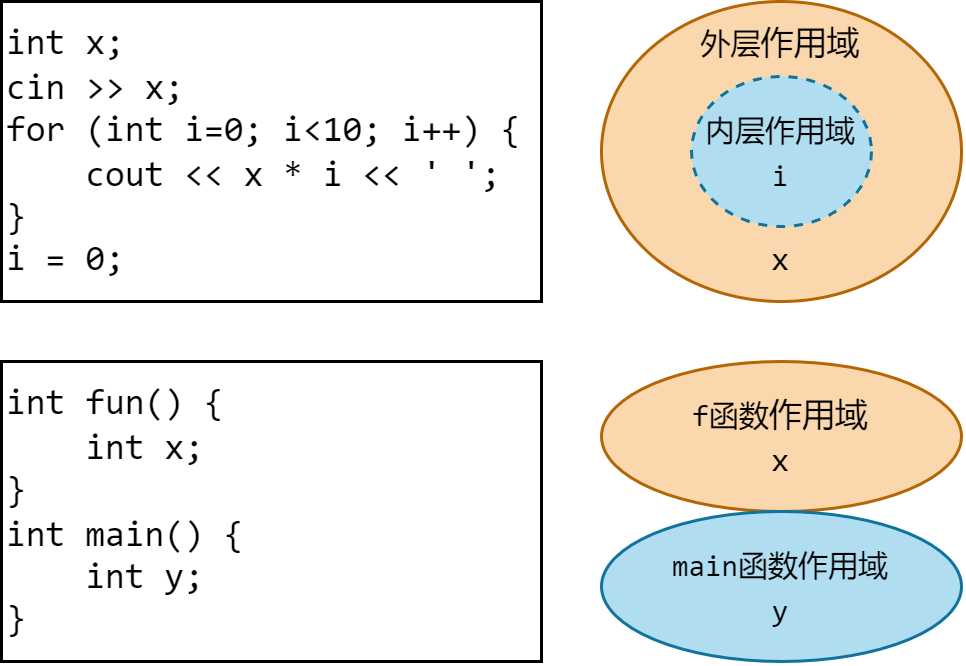
\includegraphics[width=0.6\textwidth]{../images/generalized_parts/04_block_scope_and_function_scope_300.png}
    \caption{块作用域与函数作用域的区别}
\end{figure}
这种关系有点像是动物园。在动物园中,每个动物(局部变量)都被关在自己的围栏(函数作用域)内生活,而其它围栏内的动物不能和它们互相接触。动物饲养员则像全局变量,它可以进入各个围栏内部。\par
那么假如我需要在两个函数中传递信息(比如,在主函数中告诉 \lstinline@f@ 函数,需要求哪个数的绝对值),我该怎么办呢?这时就需要用到参数传递和返回值了。\par
\subsection*{实参与形参}
回顾一下我们刚才写的自定义绝对值函数 \lstinline@f@ 。
\begin{lstlisting}
double f(double x) { //返回类型为double,接收一个double型参数x
    if (x >= 0) { //如果x>=0,返回x本身
        return x;
    }
    else { //如果x<0,返回x的负值
        return -x;
    }
}
\end{lstlisting}
这里的 \lstinline@x@ 是它的一个参数。我们在调用 \lstinline@f@ 时,程序会新定义一个 \lstinline@x@,而括号内的数据会作为初始化信息传递给 \lstinline@x@。举例说,\lstinline@f(-.1)@ 在主函数中被调用,这时程序会新定义一个 \lstinline@x@ 并初始化为 \lstinline@-.1@,然后开始顺序执行 \lstinline@f@ 中的代码。换言之,每次调用 \lstinline@f@,程序都会重新定义一个 \lstinline@x@,所以我们可以把参数列表当作是``函数中的一种变量定义语句''。\par
那么如果我把这个函数中的所有 \lstinline@x@ 都换成 \lstinline@y@,这个函数的本质发生变化了吗?
\begin{lstlisting}
double f(double y) { //返回类型为double,接收一个double型参数y
    if (y >= 0) { //如果y>=0,返回y本身
        return y;
    }
    else { //如果y<0,返回y的负值
        return -y;
    }
}
\end{lstlisting}
答案当然是不会!名字是可以随便起的,无论用 \lstinline@x@ 还是 \lstinline@y@,还是换成 \lstinline@num@ 或者 \lstinline@arg@,都没问题。但是,只要函数的逻辑不变,它的本质就没有发生变化,对于相同的输入,永远会给出相同的输出。数学上也是如此,对于相同的定义域来说,$f(x)=\left|x\right|$和$f(y)=\left|y\right|$当然是同一个函数。\par
真正会改变函数值的不是参数的名字,而是具体传入函数的输入信息。\lstinline@f(3)@ 和 \lstinline@f(4)@ 当然是不同的;\lstinline@f(3)@ 和 \lstinline@f(-3)@ 虽然相同,但它们传递的信息还是有差异的,只是输出恰好一致。所以说,同样是``参数'',\lstinline@x@ 或 \lstinline@y@ 仅仅代表一个名字,而 \lstinline@3@ 或 \lstinline@4@ 却能传递真正有效的信息,看来它们还是有一定的区别的。\par
我们把 \lstinline@x@ 和 \lstinline@y@ 这类\textbf{在函数定义过程中用到的名字称为形参(Parameter/Argument)},而把 \lstinline@3@ 和 \lstinline@4@ 这类\textbf{在函数调用过程中传递了真实信息的数据称为实参(Argument/Parameter)}。\footnote{parameter和argument这两个词都可以用来指代参数。不过习惯上,parameter指代形参,而argument指代实参。}请注意,实参未必就``没有名字'',它可以是字面量、常量表达式、常量或变量;形参和实参的区别应该在于:你是在定义还是在调用。\par
\subsection*{函数的使用}
举个例子,现在我们要写一个 \lstinline@max@ 函数,它可以接收两个整数输入,返回值是其中较大的那个整数。\par
首先确定返回类型和参数。这个函数只需接收整数参数,返回整数值,所以返回类型可以是任何一种整型,具体哪种就看我们需要了。为了能涵盖比较大的数据范围,我们在这里可以选择 \lstinline@long long@。我们需要两个参数,它们都是 \lstinline@long long@ 类型的。名字可以随便起,比如 \lstinline@a@ 和 \lstinline@b@ 吧。\par
函数体内的部分需要返回 \lstinline@a@ 和 \lstinline@b@ 的较大值,这就需要我们分析一下如何实现:如果 \lstinline@a@ 大于 \lstinline@b@,那我们就返回 \lstinline@a@,这没问题;如果 \lstinline@a@ 不大于 \lstinline@b@,那我们就返回 \lstinline@b@,也不会出错。所以我们需要一个选择结构。我们可以这么写:
\begin{lstlisting}
long long max(long long a, long long b) {
    //接收两个long long参数,给出long long返回值
    if (a > b) { //当a>b时返回a
        return a;
    }
    else { //否则返回b
        return b;
    }
}
\end{lstlisting}\par
接下来写一下主函数的部分就可以了。这是我们熟知的内容,所以我只放代码,不再讲解思路。
\begin{lstlisting}
int main() {
    long long a, b; //定义int型变量a,b
    cin >> a >> b; //输入a,b的值
    cout << max(a, b); //调用max
    return 0;
}
\end{lstlisting}
请留意:主函数中的 \lstinline@a@ 和 \lstinline@b@ 与 \lstinline@max@ 函数中的 \lstinline@a@ 和 \lstinline@b@ 是完全不同的概念。它们分别属于不同的、相互独立的作用域,互不干涉。\par
如果我们要输入三个数并找出其最大值呢?一种方法是,先用 \lstinline@max@ 求出其中两数的最大值,然后再求出它和第三个数的最大值。
\begin{lstlisting}
int main() {
    long long a, b, c; //定义三个int型变量a,b,c
    cin >> a >> b >> c; //输入a,b,c的值
    cout << max(max(a, b), c); //输出它们三个的最大值
}
\end{lstlisting}
我们来解析一下 \lstinline@max(max(a,b),c)@ 这段代码,不难:\par
首先,\lstinline@max(a,b)@ 先行计算,返回的是 \lstinline@a@, \lstinline@b@ 中的最大值。这个返回值又作为 \lstinline@max@ 的参数与 \lstinline@c@ 比较,最后返回的就是 \lstinline@a@, \lstinline@b@, \lstinline@c@ 中的最大值。\par
当然还有别的方法,我们也可以定义一个 \lstinline@max3@ 函数\footnote{我们很快就会讲到重载,那时就可以直接重载一个 \lstinline@max@ 函数。},接收三个参数并求出它们的最大值。
\begin{lstlisting}
long long max3(long long a, long long b, long long c) {
    //接收三个long long参数,给出long long返回值
    const long long max_ab {max(a,b)}; //先求出a,b的最大值
    if (max_ab > c) { //如果a,b的最大值大于c,返回前者
        return max_ab;
    }
    else { //否则返回后者
        return c;
    }
}
\end{lstlisting}
这样我们就可以用 \lstinline@max3@ 函数来求三个数的最大值了。\par
初学者可能有这样的误会,认为只有主函数才能调用其它函数。不是的,所有函数都可以调用其它函数,只要有声明(我们稍后谈到)。函数可以调用它自身,这就是递归\footnote{我们会在后面的内容中讲到递归。}。其它函数甚至可以调用主函数,但这往往容易引起困惑,所以我不推荐这么做。\par
如果涉及大量数据求最大值的问题,这种方法就显得不太合适,这时我们可能考虑寻求 \lstinline@valarray@ 等其它方案,这些我们之后再谈。\par
\subsection*{函数的声明}
有些程序员在写代码的时候更倾向于把主函数写在靠前的位置上,这样一来,程序的主要操作是什么就一目了然——毕竟,主函数是程序开始执行的地方。\par
不过如果单纯只是这么写的话,编译器就会报错。以下是例子:
\begin{lstlisting}
int main() {
    long long a, b, c; //定义long long型变量a,b,c
    cin >> a >> b >> c; //输入a,b,c的值
    cout << max3(a, b, c); //输出a,b,c的最大值
//error: 'max3' was not declared in this scope
}
long long max(long long a, long long b) {
    //省略
}
long long max3(long long a, long long b, long long c) {
    //省略
}
\end{lstlisting}
编译器报错信息的含义是:``\lstinline@max3@ 在这个作用域中没有定义。''读者可能会误会,认为把 \lstinline@max3@ 定义在 \lstinline@main@ 函数中就可以了。但是,传统意义上的\textbf{一个函数不能定义在其它函数当中,而必须定义在全局作用域中}\footnote{我们在精讲篇中会介绍lambda闭包,它是一种可以在局部作用域中定义的函数。}!这些函数之间的关系是并列的,而非 \lstinline@max3@ 从属于 \lstinline@main@。\par
Visual C++编译器返回的报错信息更清晰:``\texttt{error C3861: 'max3': identifier not found}。''它的意思是:``没有找到 \lstinline@max3@ 这个标识符。''这是因为,编译器处理代码是从前向后处理的。它遇到一个函数声明(或定义)就会记住;然后一旦遇到函数调用,就去寻找能匹配这个调用的函数。现在我们把 \lstinline@max3@ 的调用放在前,而 \lstinline@max3@ 的定义放在后,那么编译器自然会``not found''了。\par
我们既想要把长篇累牍的函数体放在后面以突出重点(主函数),又不得不在主函数之前把``存在这样一个函数''的信息告诉编译器,那么最好的解决方案就是\textbf{声明(Declaration)}了。\par
所谓函数的声明,就是把一个函数的外部特征告诉编译器,这样编译器就可以在调用相应函数时匹配到它。至于这个函数会做什么,先不要管它,等到\textbf{定义(Definition)}中再告诉编译器。\par
声明一个函数的基本语法是
\begin{lstlisting}
<返回类型> <函数名>(<参数类型列表>); //注意用分号结尾
\end{lstlisting}
简单说来就是,把花括号包起来的函数体部分去掉,然后用一个分号结束该句即可。\par
在函数声明的语法中,我们只需要列出参数的类型,而不需要指明参数的名称——它只是个形参而已,定义成什么名字其实无所谓,而且我们又无需在函数体(因为没有写)中使用它,所以仅仅指明类型,让编译器知道它该接收什么参数就足够。\par
如果我们要为前面定义的 \lstinline@f@ 写一个声明,可以这么写:
\begin{lstlisting}
double f(double); //形参名可省略,或者任意取名
\end{lstlisting}
如果我们要为 \lstinline@max@ 和 \lstinline@max3@ 写声明,可以这么写:
\begin{lstlisting}
long long max(long long, long long); 
long long max3(long long, long long, long long);
\end{lstlisting}\par
所以我们把代码整理一下,就可以形成一个完整的程序:
\begin{lstlisting}[caption=\texttt{max3.cpp},label=lst:max3]
//这个程序可以接收三个输入整数,并给出它们的最大值
#include <iostream> //标准输入输出头文件
using namespace std; //使用命名空间std
long long max3(long long, long long, long long); //声明
int main() {
    long long a, b, c; //定义long long型变量a,b
    cin >> a >> b >> c; //输入a,b的值
    cout << max3(a, b, c); //输出a,b,c的最大值
    return 0;
}
long long max(long long a, long long b) {
    //接收两个long long参数,给出long long返回值
    if (a > b) { //当a>b时返回a
        return a;
    }
    else { //否则返回b
        return b;
    }
}
long long max3(long long a, long long b, long long c) {
    //接收三个long long参数,给出long long返回值
    const long long max_ab {max(a,b)};
    if (max_ab > c) { //如果a,b的最大值大于c,返回前者
        return max_ab;
    }
    else { 否则返回后者
        return c;
    }
}
\end{lstlisting}
这里有个问题需要读者留意:为什么这里只需要声明 \lstinline@max3@ 而不需要声明 \lstinline@max@ 呢?其原因在于,\lstinline@max@ 是在 \lstinline@max3@ 中调用的,而 \lstinline@max@ 的定义在 \lstinline@max3@ 之前,所以编译器不会找不到 \lstinline@max@,参见图4.3的蓝色箭头。\par
\begin{figure}[htbp]
    \centering
    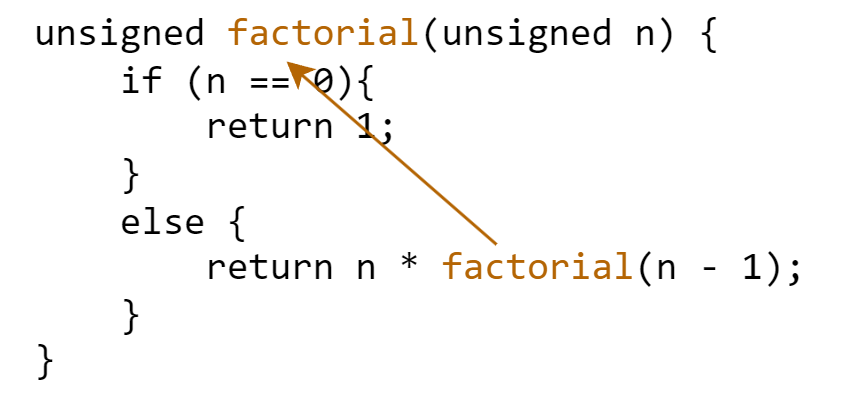
\includegraphics[width=0.8\textwidth]{../images/generalized_parts/04_max3_code_logic_300.png}
    \caption{\lstinline@main@ 函数调用了 \lstinline@max3@,而 \lstinline@max3@ 调用了 \lstinline@max@,它们都能够找到对应的函数}
\end{figure}
这也就是说,其实 \lstinline@main@ 函数没有调用 \lstinline@max@,调用 \lstinline@max@ 的其实是 \lstinline@max3@。这种关系对于初学者来说可能相当复杂,不过即使现在很难理解也没有关系,我们在日后的学习过程中会慢慢体会到的。\par
\subsection*{``值计算''与``副作用''}
用函数的视角来理解运算符是一种很重要的思想。C++中的自增/自减运算符可以当作一个函数来看待,它接收某个类型(实际上它可以接收很多类型)的参数,然后返回同类型的参数。如果用于后缀形式,它的返回值是原数;如果用于前缀形式,它的返回值是原数加/减 \lstinline@1@ 后的值\footnote{这里忽略整数溢出和浮点精度问题。}。\par
然而它的作用不仅仅停留在``提供一个返回值'',它还有改变原数(参数)的功能。自增/自减作用于某个变量,会导致这个变量增加/减少 \lstinline@1@。这类功能不是通过返回值表现出来的,我们称它为\textbf{副作用(Side effect)};而对应地,把通过返回值表现出来的功能称为\textbf{值计算(Value computation)}。\par
有些时候,比如在 \lstinline@for@ 循环的迭代操作中,我们使用自增/自减运算符是为了使用它的副作用,而不是值计算。对于函数来说也是同理。还记得我之前提供的 \lstinline@input_clear@ 函数吗?它的返回类型是 \lstinline@void@(空),我们不需要接收它的什么返回值,而只需要使用它的副作用(清除错误状态,清除本行输入)就行。
\begin{lstlisting}
void input_clear() {
    cin.clear(); //清除错误状态
    while (cin.get() != '\n') //清除本行输入
        continue;
}
\end{lstlisting}
我们还会自定义很多这类的``只用其副作用而不用其值''的函数,这种情况下我们可以将返回类型定为 \lstinline@void@。\lstinline@void@ 函数中可以写 \lstinline@return ;@ 或者 \lstinline@return void{};@\footnote{\lstinline@void{}@相当于一个 \lstinline@void@ 类型的临时对象,我们会在后面经常遇到这类语法的。}这样的返回语句,或者压根什么返回语句也不写,没有问题。\par
